\documentclass[a4paper,12pt]{article}
\usepackage{graphicx}
\usepackage{xcolor}
\usepackage{polski}
\usepackage{multicol}
\usepackage{url}

\title{
	Projekt gry sieciowej wykorzystującej szyfrowanie RSA \\
	Technologie Telekomunikacyjne}
\author{Jakub Zając, Marcin Klocek}
\date{December 2024}

\begin{document}

\maketitle

\section{Opis projektu}
W ramach projektu została opracowana gra Kółko i Krzyżyk.
Gracze łączą się z serwerem, który umożliwia gre przez internet.
Po nawiązaniu połączenia, następuje przekazanie kluczy publicznych przez
obie strony co zapewnia szyfrowanie RSA.
W trakcie gry dane wymieniane są za pomocą protokołu TCP/IP.
Całość jest zaimplementowana w języku \texttt{Python}

\section{RSA/Padding OAEP}
\subsection{RSA}
Do szyfrowania użyty został protokół RSA z kluczem 1024-bitowy.
Zgodnie ze specyfikacją algorytmu szyfrowanie zostaje przeprowadzane
poprzez mnożenie modularne: \newline

\begin{multicols}{2}
\begin{center}
\Large Szyfrowanie \newline
\Large $ c~=~m^e~\mathrm{mod} ~ n$
\end{center}
\vfill

\begin{center}
\Large Deszyfrowanie \newline
\Large $ m~=~c^d~\mathrm{mod} ~ n$
\end{center}
\vfill
\end{multicols}
Gdzie \textit{c} to wiadomość zaszyfrowana w postaci liczby
całkowitej z zakresu  1 $\cdots$ \textit{n}, gdzie n to
liczba większa od $2^{1023-1}$, \textit{e} - klucz publiczny
oraz \textit{d} klucz prywatny. Program za każdym razem losuje
dwie liczby pierwsze wystarczająco duże by ich iloczyn dał
w wyniku liczbe \textit{n}. Trudność złamania szyfry
polega na trudności faktoryzacji \textit{n}.

\newpage
\subsection{Padding}
Aby zapewnić danym odpowiednią długość (przy zbyt małej długości
bitowej danych szyfr może zostać łatwo złamany) stosujemy
\textit{Optimal asymmetric encryption padding}, który odpowiednio wydłuży dane.
Algorytm ten wykorzystuje hashowanie \texttt{SHA-256}  oraz funkcje \texttt{mgf1}.
Dodatkowo każdorazowo przy padding'owniu losowany jest nowy \textit{seed}
używany podczas tego procesu. W naszym projekcie użyłem gotowych
bibliotecznych funkcji hashujących oraz gotowej implmentacji funkcji \texttt{mgf1}.

\begin{figure}
\centerline{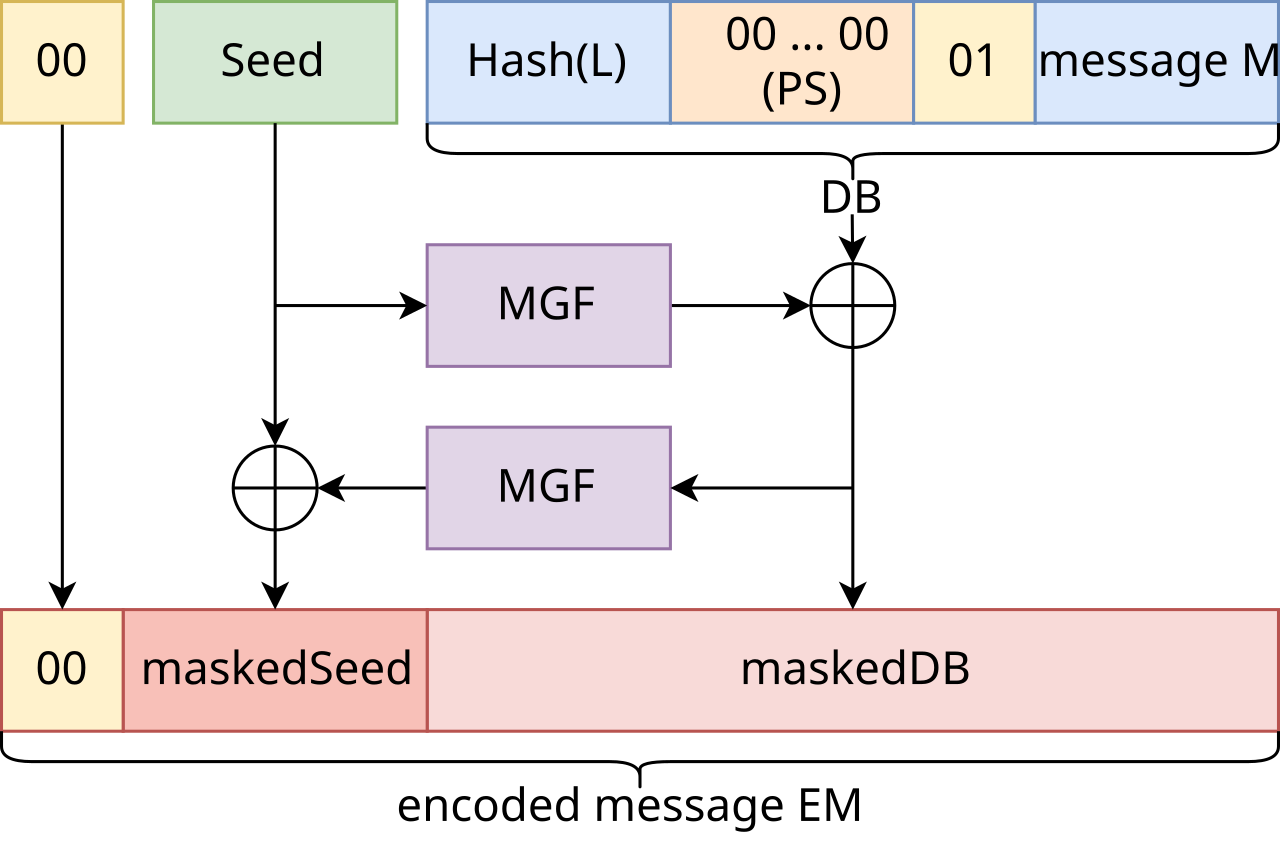
\includegraphics[scale=0.15]{OAEP.png}}
\caption{Optimal asymmetric encryption padding}
\end{figure}
Całkowita długość ramki to 128 bajtów, funkcja hashująca koduje
pusty \texttt{label = ''} do porcji 32 bajtowej, \textit{seed} również
ma 32 bajty, reszta to wiadomość oraz uzupełnienia tak jak to
widać na rysunku. Wynikowo dane mają 1024 znaki bitowe.

\newpage

\section{Detale implementacji}
\subsection{Komunikacja Serwer-Client}
Komunikacja nawiązywana jest poprzez gniazdo (\textit{socket}) za pomocą protokołu TCP/IP. Po nawiązaniu połączenia serwer-client, następuje podwójna wymiana kluczy. Zarówno klient jak i serwer ma swoją parę kluczy publicznych \textit{(d,e)} którą wymienia między sobą w przestrzeni publicznej, dzięki czemu szyfrowanie działa w obie strony.  

Nawiązanie połączenia przebiega następująco: 
\begin{enumerate}
	\item Udostępnienie klucza publicznego przez serwer
	\item Potwierdzenie po stronie klienta
	\item Udostępnienie klucza publicznego przez klienta
	\item Potwierdzenie po stronie serwera
	\item Rozpoczęcie właściwej komunikacji
\end{enumerate}


\begin{figure}[ht]
	\centerline{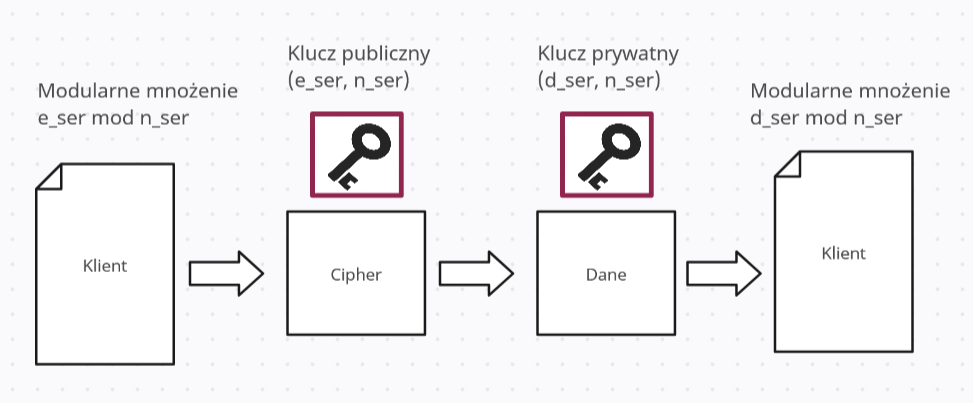
\includegraphics[scale=0.6]{ProceszSzyfrowania.png}}
	\caption{Szyfrowanie Serwer-Klient. W drugą stronę przebiega identycznie.}
\end{figure}

\subsection{GUI}

Graficzny interfejs użytkownika powstał przy użyciu biblioteki \texttt{pygame}. Jest to
biblioteka zaprojektowania specjalnie do tworzenia gier.

\subsection{Inne narzędzia wykorzystane w projekcie}

Aby ułatwić pisanie kodu, zostały użyte następujące narzędzia:

\begin{itemize}
	\item \texttt{setup-tools} - narzędzie do pakowania kodu w pakiet Pythona.
	Wymusza on odpowiednią strukture plików pakietu z czego korzystają również
	inne narzędzia. Pozwala na opisywanie zależności programu, oraz plików
	wykonywalnych dostarczanych z pakietem.
	\item \texttt{pytest} - biblioteka do pisania automatycznych testów jednostkowych.
	W projekcie spora część kodu ma odpowiednie testy, co pozwala na szybsze pisanie
	implementacji, oraz utrzymanie jakości.
	\item \texttt{mypy} - narzędzie do statycznej analizy typów w kodzie.
	\item \texttt{google protobuf} - język do opisu danych, oraz generator
	serializatorów i deserializatorów tych danych. Używany do opisu protokołu
	gry.
\end{itemize}

\section{Repozytorium}
Poniżej udostępniamy link do naszego repozytorim ze wszystkimi kodami źródłowymi.
\newline
\url{https://github.com/mklck/tt-project/tree/main}
\end{document}
